\section{Einleitung}
\label{sec:introduction}

Es gibt eine große Menge an Software, für die grafische Erstellung und Bearbeitung eines Datenbankschemata. Diese variieren von der unterstützten Datenbank, der Funktionalität und ob sie als webbasierte Software, eigenständige Software oder als Plugin zur Verfügung stehen.

Dabei sind die vorhandenen Programme meist an Benutzer gerichtet, die bereits Wissen über das Thema Datenbanken besitzen. 
Dadurch enthalten die Programme möglichst viele Funktionen, die von der jeweiligen Datenbank unterstützt werden. Das Erlenen der Thematik mit Hilfe solcher Software, erweist sich häufig als hinderlich. Anfänger erhalten eine Software, welche eine große Menge an Funktionen besitzt, für die bereits Wissen vorhanden sein muss.

Die Bedienbarkeit ist dabei im Fokus. Funktionen führen zusätzliche Aktionen aus, die notwendig und als selbstverständlich für erfahrene Benutzer sind. Für Anfänger ist dabei aber nicht direkt ersichtlich welche Aktionen getätigt wurden, und aus welchem Grund diese notwendig sind.

Dabei vorab zu erwähnen ist die Software ``MySQL Workbench'', die im Abschnitt~\ref{sec02:mysql_workbench} noch genauer beschrieben wird. MySQL Workbench ist eine Software, von Profis an Profis. Studenten die mit dieser Software ihre ersten Schritte zum Thema Datenbanken machen, stellen sich die Frage, welche der beiden zur Verfügung gestellten Knöpfe benutzt werden müssen zum Erstellen der Foreign Keys~\footnote{Fremdschlüssel}, anstelle der Überlegung was der Unterschied der Foreign Keys für die Datenbank bedeutet.

Mit dieser Arbeit wird versucht eine Lernsoftware zu entwickeln, die an Anfänger gerichtet ist. Es sollen die elementaren Funktionen zur Erstellung von Datenbanken zur Verfügung gestellt werden. Dabei sollen Fehler  nicht von der Software automatisch gelöst werden, sondern an den Benutzer kommuniziert werden. Somit der Benutzer ein Verständnis dafür bekommt, welche Bedingungen vorher erfüllt sein müssen, um die jeweilige Aktion durchzuführen.

Eine bereits vorhandene Lernsoftware namens ``Blattwerkzeug''~\ref{subsec03:bereits_vorhanden_projekt} wurde als Master Thesis an der Fachhochschule Wedel, von Marcus Riemer entwickelt. Blattwerkzeug ist für den Schulunterricht gestaltet worden und richtet sich an eine junge Zielgruppe~\ref{subsubsec03:zielgruppe}, mit der die Entwicklung von Webseiten unter der Verwendung von Datenbanken gelehrt werden soll. 

Dadurch wurde diese Arbeit als Erweiterung der Software Blattwerkzeug entwickelt. Somit kann vom Benutzer nachdem dieser das Erstellen einer Datenbank gelernt und angewendet hat, die Datenbank in einem praktischen Umfeld und zum zusätzlichen lernen anderer Themen verwenden.

Die in dieser Arbeit entwickelte Erweiterung, ermöglicht es ein komplett neues Schema zu erstellen. Das Schema, die einzelnen Tabellen und auch die in den Tabellen enthaltenen Daten können damit angezeigt werden. Zusätzlich lassen sich die Tabellen nach dem Erstellen in einem Editor verändern. \\
Die Darstellung der Erweiterung ist in den folgenden Bildern (\ref{pic:schema_preview} und \ref{pic:table_editor_preview}) dargestellt:

\begin{figure}[ht]
    \frame{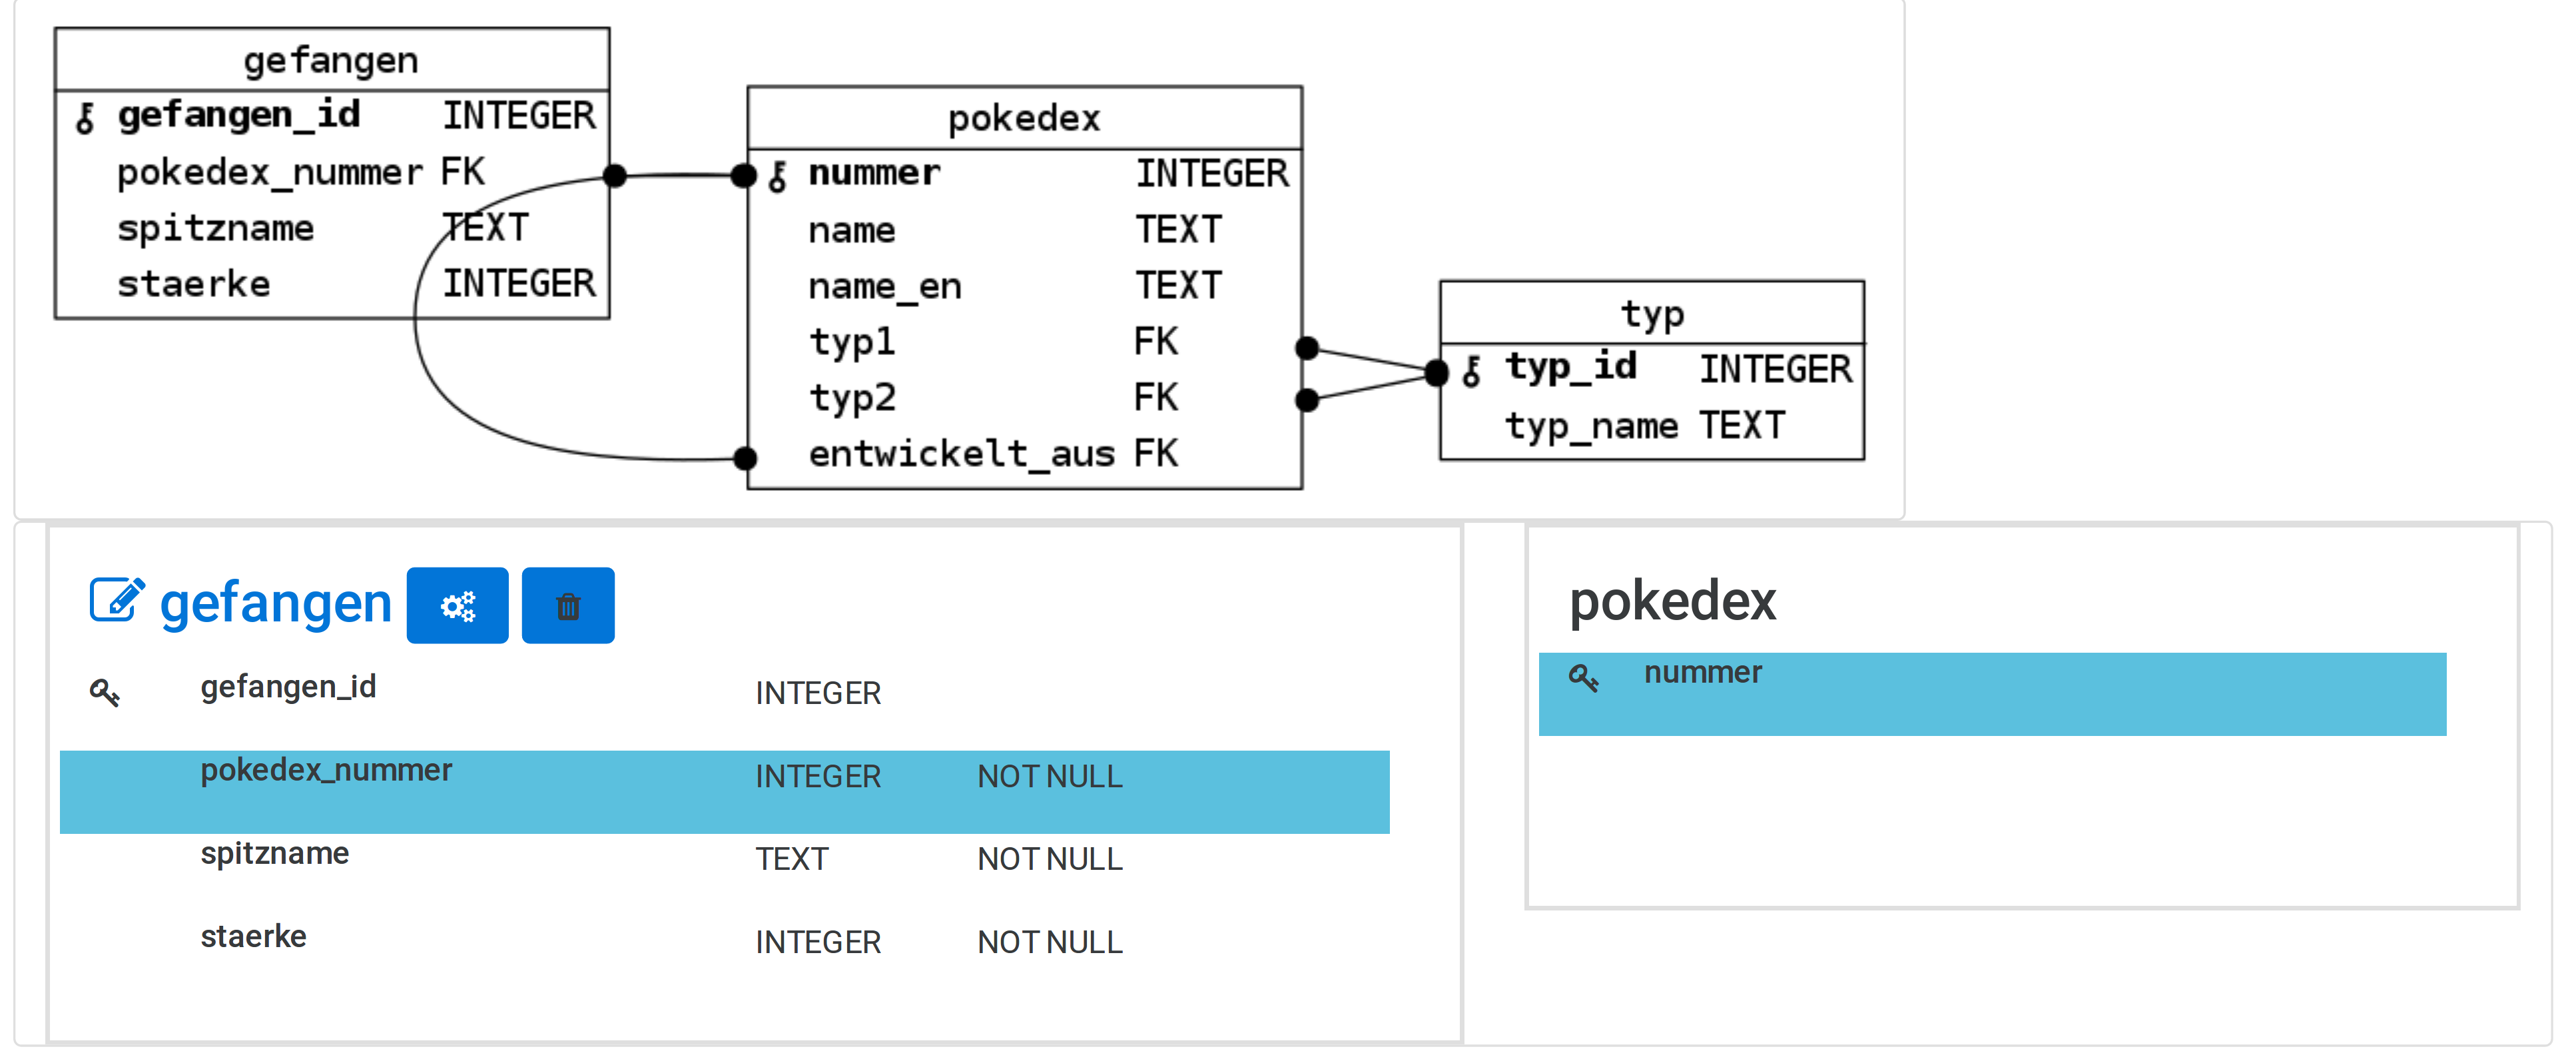
\includegraphics[width=\textwidth]{images/kap-1-schema.png}}
        \centering
        \caption{Darstellung des Schemas}
        \label{pic:schema_preview}
\end{figure}

\begin{figure}[ht]
    \frame{\includegraphics[width=\textwidth]{images/kap-1-editor.png}}
        \centering
        \caption{Tabellen Editor}
        \label{pic:table_editor_preview}
\end{figure}



In der folgenden Ausarbeitung werden die einzelnen Schritte der Entwicklung, die Gedankengänge dabei und die entstandenen Funktionalitäten genau beschrieben. \\
In einer ersten Übersicht~\ref{sec02:vergleichbare_arbeiten} werden einige verschiedenen Programmen vorgestellt, die einen ähnlichen Nutzen haben wie diese Erweiterung. Dabei werden die vorhanden Funktionen und die Bedienung der einzelnen Programme genauer betrachtet.\\
In den nachfolgenden Kapiteln wird der genaue Prozess der Entwicklung beschrieben. Dabei wird erst die Struktur von Blattwerkzeug genauer betrachtet~\ref{subsec03:bereits_vorhanden_projekt} und welche Funktionalitäten dadurch entwickelt werden sollten.~\ref{subsec03:was_benoetigt}.
In einer detaillierten Beschreibung wird genau erläutert wie die einzelnen Komponenten der Erweiterung implmentiert wurden. Dabei wird vom Client~\ref{subsec04:client_viz} bis hin zum Server~\ref{subsec04:server} die einzelnen Aspekte genau beschrieben. \\
Im letzten Kapitel Fazit~\ref{sec05:fazit} wird noch einmal Revue passiert was letzten Endes entwickelt wurde. Welche Komponenten und aus welchen Gründen nicht implementiert werden konnten. Für weitere zusätzliche Entwicklung an der Software, werden einzelne Möglichkeiten aufgelistet, die während der Bearbeitung dieser Arbeit aufgekommen sind.

\warning[Hinweis]{Der aktuelle Stand von Blattwerkzeug kann sich auf der Seite \url{http://www.blattwerkzeug.de/} angeschaut und ausprobiert werden. Für eine Einführung zur Benutzung, der in dieser Arbeit entstandenen Erweiterung, ist im Anhang~\ref{sec:attachment} die Erstellung eines Beispielschemata beschrieben, welches der praxisorientierte Leser nachbauen kann.} 
